\section{Observational case studies}
\label{sec:case-studies}

In observational studies of bow-shaped arcs around OB stars, it is
frequently assumed that all such objects are wind-supported bow shocks
(e.g., \citealp{Kobulnicky:2016a}). Our results from
\S~\ref{sec:strong-gas-grain} show that this is indeed a fair
assumption in the absence of gas-grain decoupling, so long as the
ambient density is less than about \SI{100}{cm^{-3}} (see
Fig.~\ref{fig:zones-v-n-plane}). In other words, most OB stars
interacting with the diffuse interstellar medium are probably in the
wind bow shock regime.  Therefore, to find examples of
radiation-supported bow waves and bow shocks it is necessary to look
at arcs inside \hii{} regions and star-forming clouds, where the
ambient densities are much higher.

\subsection{Evidence for radiation-supported bows}

One potentially promising sample is the Carina mid-infrared bow shocks
\citep{Sexton:2015b}.   are in a high density environment,
\SI{1000}{cm^{-3}}, so they may be bow waves.  There seems to be
spectral types for most of them: B0 (but supergiant) to O7.  Sizes are
3 to 12 arcsec, which at Carina (\SI{2.3}{kpc}) is
\SIrange{0.033}{0.134}{pc}.

Amazingly, the size/density combination gives regions that overlap
with the dust wave region for both the \SI{20}{M_\odot} and \SI{40}{M_\odot}
case.  And implying velocities of \SIrange{30}{50}{km.s^{-1}}.  This
is more believable than the \SI{10}{km.s^{-1}} that they quote, since
that would not give a shock at all.  This would imply
\(\tau > \eta \approx 0.1\), so the bow luminosity should be 10\% of the star
luminosity, so getting on for \SI{e4}{L_\odot}.

Two small bows in M42:

\newcommand{\thD}{\(\theta^1\)\,Ori~D}
\th1D{} (Ney--Allen nebula) \citep{Robberto:2005a}

LP~Ori: B1.5V star, like our \SI{10}{M_\odot} example. Radius about
\(3''\), so 0.005 pc.  With \(v = 80\) that would clearly be a dust
wave and would require \SIrange{100}{1000}{cm^{-3}}. Gaia distance \SI{408 +- 11}{pc}


Ones that Ochsendorf claims are dust waves (Narrator: they aren't).


\begin{figure*}
  \centering
  \includegraphics[width=\linewidth]{figs/orion-LP-and-th1D-color}
  \caption{Bows driven by the OB stars \thD{} and LP~Ori in the Orion
    Nebula.  (a)~Large-scale infrared view of the Orion Molecular
    Cloud.  Red, green, and blue intensity show respectively Herschel
    PACS observations at \SIlist{160; 70}{\um}, and Spitzer IRAC
    observations at \SI{8}{\um}.  Red traces thermal emission from
    cool dust (\(T < \SI{30}{K}\)) in the dense molecular filament.
    Green traces thermal emission from warmer dust
    (\(T \approx \SI{40}{K}\)) in the neutral PDR, which is heated by
    far-ultraviolet radiation from the OB stars in the cluster. Blue
    traces emission from PAH \SIlist{7.6;7.85}{\um} bands in the same
    neutral PDR plus thermal emission from hotter dust
    (\(T > \SI{100}{K}\)), which is found inside the ionized \hii{}
    region.  (b)~Zoom on the central parsec of the Orion Nebula (M42),
    showing short-wavelength mid-infrared emission from Spitzer IRAC
    observations (\SIlist{8.0;5.8;4.5}{\um}).  Red shows the same as
    blue in panel~a.  Green show predominantly the \SI{6.2}{\um} PAH
    band.  Blue shows mainly stellar photospheric emission, plus a
    minor contribution due to the Br~\(\alpha\) emission line from ionized
    gas. Some major components of the nebula are labelled: the
    Trapezium cluster, which contains the majority of the massive
    stars; the Kleinmann-Low reflection nebula, illuminated by massive
    stars embedded in the molecular filament; the Orion Bar, a
    prominent edge-on ionization front and PDR.  (c)~Zoom on the
    central \SI{0.1}{pc} of the Trapezium cluster, showing longer
    wavelength mid-infrared emission from UKIRT MAX
    (\SIlist{19.7;10.1}{\um}).  In this central zone, these
    wavelengths (shown in red and green) are dominated by warm
    (\SIrange{100}{300}{K}) silicate grains, while the IRAC
    \SI{5.8}{\um} emission (blue) shows stellar photospheres and the
    very warmest dust.}
  \label{fig:orion-bows}
\end{figure*}

\begin{figure*}
  \centering
  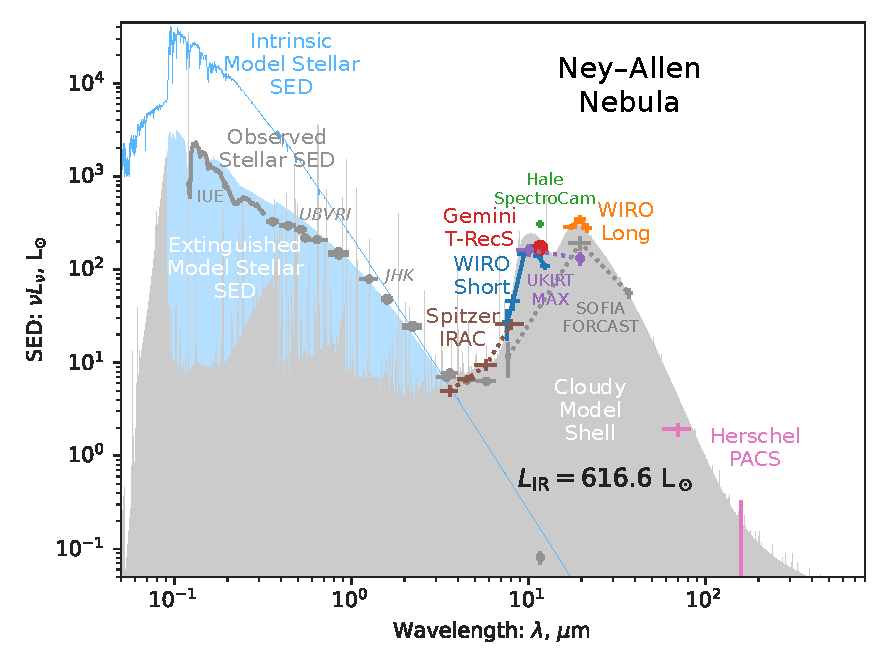
\includegraphics[width=\linewidth]{figs/ney-allen-sed-edited}
  \caption{Ultraviolet-to-infrared spectral energy distribution of the Ney--Allen
    nebula that surrounds \thD. }
  \label{fig:ney-allen-sed}
\end{figure*}


\begin{figure*}
  \centering
  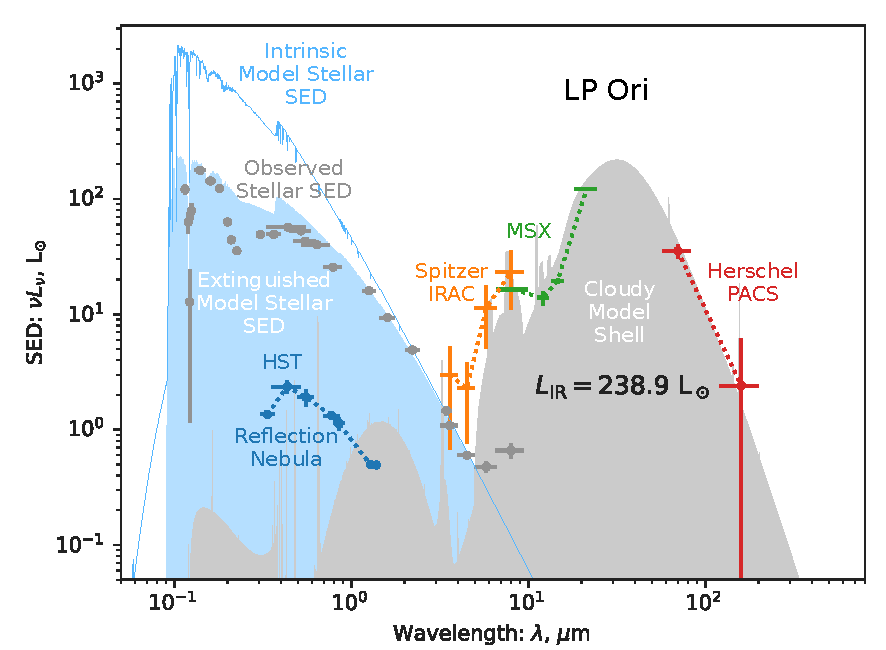
\includegraphics[width=\linewidth]{figs/lp-ori-sed-edited}
  \caption{Ultraviolet-to-infrared spectral energy distribution of LP~Ori
    and associated nebula. }
  \label{fig:lp-ori-sed}
\end{figure*}

\begin{figure}
  \centering
  \includegraphics[width=\linewidth]{figs/lp-ori-wfpc2-continuum-subtract}
  \caption{Narrow-band images of LP Ori nebula }
  \label{fig:lp-ori-sed}
\end{figure}

% Model shell-R001-n27-LP_Ori20Bz5 from cloudy-dust-charging
The Cloudy model for LP Ori


%%% Local Variables:
%%% mode: latex
%%% TeX-master: "two-orions-bow"
%%% End:
